\documentclass[onecolumn]{article}

\usepackage{graphicx}% Include figure files
\usepackage{bm}% bold math
\usepackage{amsmath}
\usepackage{amssymb}
\usepackage[labelfont=bf]{caption}
\usepackage[para]{threeparttable}
\usepackage[superscript,biblabel]{cite}
\usepackage{siunitx}
%\usepackage[showframe]{geometry}
\usepackage{textcomp} %Used to get centred tilde with $\sim$
\usepackage{gensymb} %\degree, avoids $^\circ$
\usepackage{float}
\usepackage[perpage,symbol*,para]{footmisc} %Symbolic footnotes
\usepackage{cuted} %Allows use of \strip for single column maths in twocolumn layout.
\usepackage{breqn}

\usepackage{geometry}
\geometry{margin=1in}

\usepackage{tikz}
\usetikzlibrary{optics}
\usetikzlibrary{arrows}
\usetikzlibrary{calc}
\usetikzlibrary{snakes}

\setcounter{MaxMatrixCols}{20}

\newcommand\scalemath[2]{\scalebox{#1}{\mbox{\ensuremath{\displaystyle #2}}}}

\graphicspath{{./Figures/}}

\begin{document}

\begin{figure}[h]
\centering
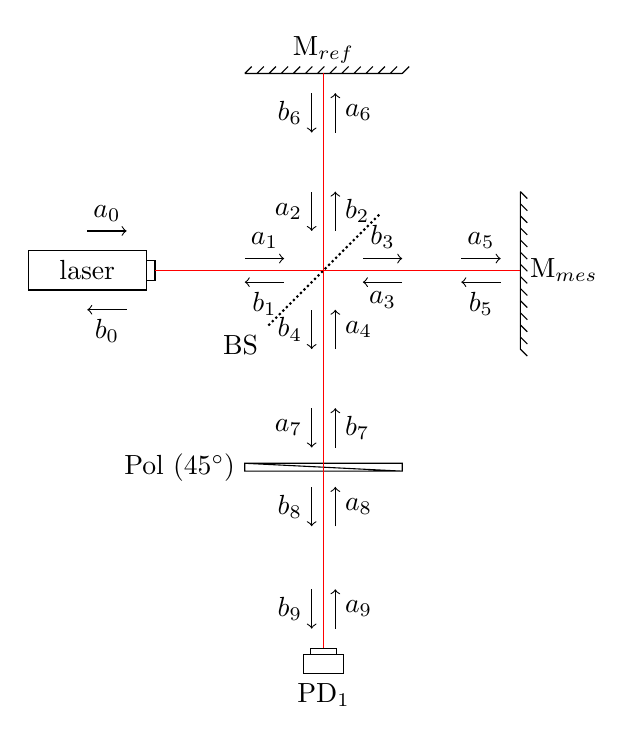
\begin{tikzpicture}[use optics] 
	%\draw[style=help lines,gray!50] (-6cm,-6cm)grid[step=0.5cm] (6cm,6cm);
	\node[semi-transparent mirror,rotate=-45] at (0,0) (bs) {};	
	\node[mirror] at (2.5,0) (mmes) {};
	\node[mirror,rotate=90] at (0,2.5) (mref) {};
	\node[laser] (S) at (-3,0) (laser) {laser};
	\node[generic sensor, io body height = 0.5cm, rotate=-90] (S) at (0,-5) (pd1) {};
	\node[polarizer,object aspect ratio=0.05, rotate=90] (S) at (0, -2.5) (pol_o1) {};

	\draw[red] (laser.east) -- (bs.center);
	\draw[red] (bs.center) -- (mref.center);
	\draw[red] (bs.center) -- (mmes.center);
	\draw[red] (bs.center) -- (pd1.west);
	
	\draw[->] (-3,0.5) -- node[above] {$a_0$} (-2.5,0.5);
	\draw[->] (-2.5,-0.5) -- node[below] {$b_0$} (-3,-0.5);
	
	\draw[->] (-1,0.15) -- node[above] {$a_1$} (-0.5,0.15);
	\draw[<-] (-1,-0.15) -- node[below] {$b_1$} (-0.5,-0.15);

	\draw[->] (0.15,0.5) -- node[right] {$b_2$} (0.15,1);
	\draw[<-] (-0.15,0.5) -- node[left] {$a_2$} (-0.15,1);

	\draw[->] ($(mref.center) + (0.15,-0.75)$) -- node[right] {$a_6$} ($(mref.center) + (0.15,-0.25)$);
	\draw[<-] ($(mref.center) + (-0.15,-0.75)$) -- node[left] {$b_6$} ($(mref.center) + (-0.15,-0.25)$);

	\draw[->] ($(bs.center) + (1,-0.15)$) -- node[below] {$a_3$} ($(bs.center) + (0.5,-0.15)$);
	\draw[<-] ($(bs.center) + (1,0.15)$) -- node[above] {$b_3$} ($(bs.center) + (0.5,0.15)$);

	\draw[->] ($(mmes.center) + (-0.75,0.15)$) -- node[above] {$a_{5}$} ($(mmes.center) + (-0.25,0.15)$);
	\draw[<-] ($(mmes.center) + (-0.75,-0.15)$) -- node[below] {$b_{5}$} ($(mmes.center) + (-0.25,-0.15)$);

	\draw[->] ($(bs.center) + (0.15,-1)$) -- node[right] {$a_4$} ($(bs.center) + (0.15,-0.5)$);
	\draw[<-] ($(bs.center) + (-0.15,-1)$) -- node[left] {$b_4$} ($(bs.center) + (-0.15,-0.5)$);

	\draw[->] ($(pol_o1.center) + (0.15,-0.75)$) -- node[right] {$a_{8}$} ($(pol_o1.center) + (0.15,-0.25)$);
	\draw[<-] ($(pol_o1.center) + (-0.15,-0.75)$) -- node[left] {$b_{8}$} ($(pol_o1.center) + (-0.15,-0.25)$);
	\draw[->] ($(pol_o1.center) + (-0.15,0.75)$) -- node[left] {$a_{7}$} ($(pol_o1.center) + (-0.15,0.25)$);
	\draw[<-] ($(pol_o1.center) + (0.15,0.75)$) -- node[right] {$b_{7}$} ($(pol_o1.center) + (0.15,0.25)$);

	\draw[->] ($(pd1.west) + (0.15,0.25)$) -- node[right] {$a_{9}$} ($(pd1.west) + (0.15,0.75)$);
	\draw[<-] ($(pd1.west) + (-0.15,0.25)$) -- node[left] {$b_{9}$} ($(pd1.west) + (-0.15,0.75)$);

	\node[below left] at (bs.south) {BS};

	\node[above] at (mref) {M$_{ref}$};
	\node[right] at (mmes) {M$_{mes}$};
	\node[below] at (pd1.east) {PD$_1$};
	\node[left] at (pol_o1.north) {Pol (\ang{45})};
\end{tikzpicture}
\end{figure}

\end{document}
